\section{Анализ предметной области}
\label{sec:domain}

В данном разделе будет произведён обзор предметной области задачи, решаемой в рамках дипломного проекта.

\subsection{Теоретические основы распознавания номеров}
\label{sub:domain:theory_basics}
Задача распознавания автомобильных номерных знаков относится к тами научным областям как теория распознавания образов и обработка изображений.
Обработка изображений — любая форма обработки информации, для которой входные данные представлены изображением, например, фотографиями или видеокадрами. Обработка изображений может осуществляться как для получения изображения на выходе (например, подготовка к полиграфическому тиражированию, к телетрансляции и т. д.), так и для получения другой информации (например, распознание текста, подсчёт числа и типа клеток в поле микроскопа и т. д.). Кроме статичных двухмерных изображений, обрабатывать требуется также изображения, изменяющиеся со временем, например, видео.~\cite{image_precessing}

Всю область можно охарактеризовать как молодую, разнообразную и динамично развивающуюся. Интенсивное её изучение началось лишь в конце 1970-х гг., когда компьютеры смогли управлять обработкой больших наборов данных, какими являются изображения. И сейчас нет стандартной формулировки этой области, а многие методы и приложения всё ещё находятся на стадии фундаментальных исследований. В последнее время наблюдается повышение активности изучения области, ввиду всё большего применения её методов в коммерческих продуктах.

Теория распознавания образа — раздел информатики и смежных дисциплин, развивающий основы и методы классификации и идентификации предметов, явлений, процессов, сигналов, ситуаций и т. п. объектов, которые характеризуются конечным набором некоторых свойств и признаков.
Для оптического распознавания образов можно применить метод перебора вида объекта под различными углами, масштабами, смещениями и т. д. Для букв нужно перебирать шрифт, свойства шрифта и т. д.
Второй подход — найти контур объекта и исследовать его свойства (связность, наличие углов и т. д.)
Ещё один подход — использовать искусственные нейронные сети. Этот метод требует либо большого количества примеров задачи распознавания (с правильными ответами), либо специальной структуры нейронной сети, учитывающей специфику конкретной задачи.

Обрабатывать мы будем растровые изображения. Растровое изображение — изображение, представляющее собой сетку пикселей — цветных точек.

В целом задача распознавания автомобильного номера сводится к следующим: 
\begin{itemize}
  \item Пред-обработка изображений
  \item Поиск номерного знака
  \item Поиск отдельных символов на рамке с номером
  \item Распознавание символа
\end{itemize}

\subsection{Пред-обработка изображений}
\label{sub:domain:image_processing}
Под обработкой  изображений понимают семейство  методов  и  задач,  где  входной  и  выходной информацией  являются  изображения~\cite{misoi_clides}. Обработка изображений обычно преследует одну из следующих целей:
\begin{itemize}
  \item Улучшение качества изображения для восприятия человеком, т.е. сделать изображение лучше с субъективной точки зрения человека
  \item Улучшение изображение для восприятия компьютером, т.е. изменить изображение для упрощения последующего распознавания
\end{itemize}
Типичные задачи для обработки изображений это корректировка яркости, цветов, освещения и устранение шумов. 

Многие алгоритмы распознавания изображение показывают хорошие результаты при правильной пред-обработке а некоторые и вовсе не работают без пред обработки. В заключение отмечу что алгоритмы пред-обработки выбираются исключительно из нужд алгоритмов распознавания.

Рассмотрим алгоритмы предобработки использующиеся в работе.

\subsubsection{}
\label{sub:domain:image_processing:edges_detection}
Выделение границ.

Выделение границ (выделение краёв) — термин в теории обработки изображения и компьютерного зрения, частично из области поиска объектов и выделения объектов, основывается на алгоритмах, которые выделяют точки цифрового изображения, в которых резко изменяется яркость или есть другие виды неоднородностей.

Самым лучшим детектором границ считается детектор границ Кэнни~\cite{canny_edge_detector}. Потому как обладает следующими свойствами:
\begin{itemize}
  \item Хорошее обнаружение (устойчивость к шуму)
  \item Хорошая локализация (толщина выделенной границы получается 2 пикселя)
  \item Единственный отклик на одну границу
\end{itemize}

На рисунках \ref{fig:domain:image_processing:edges_detection:before_canny} и \ref{fig:domain:image_processing:edges_detection:after_canny} виден пример работы детектора границ Кэнни. 

\begin{figure}[ht]
\centering
    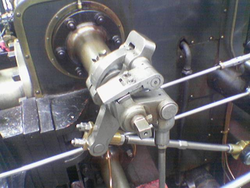
\includegraphics[scale=0.5]{before_canny.PNG}  
    \caption{Изображение до обработки детектором границ Кэнни}
    \label{fig:domain:image_processing:edges_detection:before_canny}
\end{figure}

\begin{figure}[ht]
\centering
    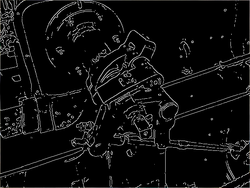
\includegraphics[scale=0.5]{after_canny.PNG}  
    \caption{Изображение после обработки детектором границ Кэнни}
    \label{fig:domain:image_processing:edges_detection:after_canny}
\end{figure}


\subsubsection{}
\label{sub:temp:image_processing:binary}
Бинаризация

Бинаризация изображений - перевод полноцветного или в градациях серого изображения в монохромное, где присутствуют только два типа пикселей (темные и светлые)\cite{binary_image}. На рисунках \ref{fig:domain:image_processing:binary:before_binarization} и \ref{fig:domain:image_processing:binary:after_binarization} виден пример бинаризации изображения.

\begin{figure}[ht]
\centering
    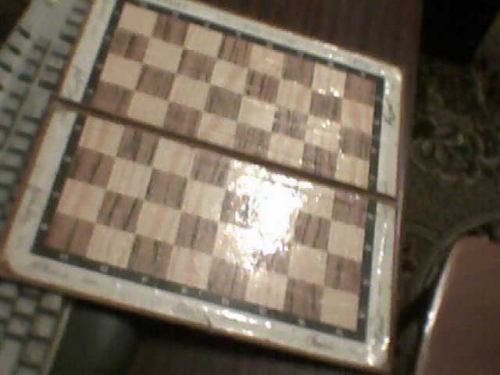
\includegraphics[scale=0.2]{before_binarization.jpg}  
    \caption{Изображение до бинаризации}
    \label{fig:domain:image_processing:binary:before_binarization}
\end{figure}
\begin{figure}[ht]
\centering
    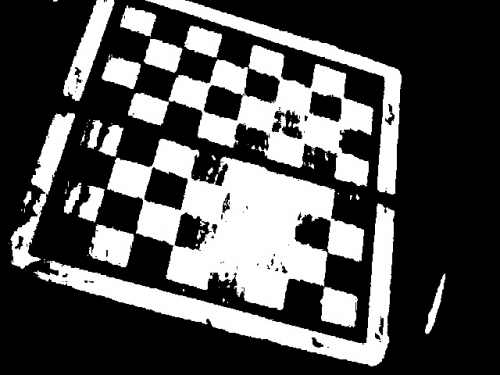
\includegraphics[scale=0.2]{after_binarization.jpg}  
    \caption{Изображение после бинаризации}
    \label{fig:domain:image_processing:binary:after_binarization}
\end{figure}

Алгоритм бинаризации несложен. Сперва требуется перевести изображение в оттенки серого использую формулу $ Y = 0.2126R + 0.7152G + 0.072B $, где Y значение градации серого, а R G и B значение каналов исходных цветов. Далее нужно сравнить значение каждого пикселя с неким пороговым значение и если значение превышает порог сделать пиксель темным и светлым если наоборот. 
Существуют различные подходы к выбору порогов, которые условно можно разделить на 2 группы:
\begin{itemize}
  \item Пороговые, которые ищут пороговое значение для изображение целиком
  \item Адаптивные, которые выбирают отдельный порог для каждого участка изображения, обычно используются при неравномерном освещении.
\end{itemize}


\subsection{Поиск номерного знака}
\label{sub:domain:search}
Рассмотрим возможные способы решения задачи поиска номерного знака.
\subsubsection{}
\label{sub:domain:search:edges_analisys}
Анализ границ и фигур.

Наиболее очевидный способ нахождение рамки это поиск прямоугольного контура. Для этого производится пред-обработка для поиска границ, например c помощью оператора Кэнни~\cite{canny_edge_detector}, затем ищутся все прямоугольники и анализируются на схожесть с государственным стандартом~\cite{stb_914_99} по соотношению сторон. Так же существует модификация~\cite{recognition_using_hought} при которой анализируется только часть рамки. Т.е. после выделения контуров ищутся вертикальные прямые и для любых прямых, расположенных недалеко друг от друга, с правильным соотношением расстояния между ними к их высоте, рассматривается гипотеза о том что номер располагается между ними. 

\begin{figure}[ht]
\centering
    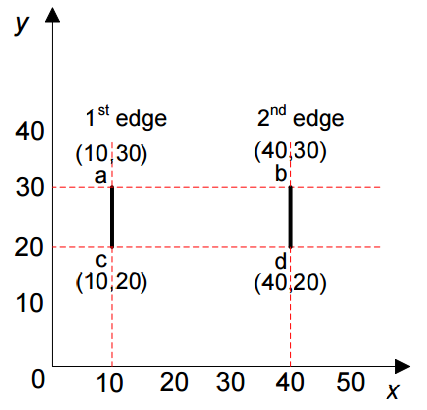
\includegraphics[scale=0.5]{edge_analysis_graphic.png}  
    \caption{Координаты боковых границ номера}
    \label{fig:domain:search:edges_analisys:edge_graphic}
\end{figure}

\begin{figure}[ht]
\centering
    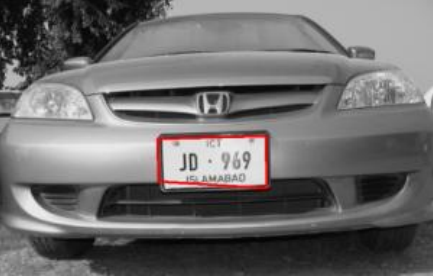
\includegraphics[scale=0.5]{edge_analysis_recognized_plate.png}  
    \caption{Распознанная граница номера}
    \label{fig:domain:search:edges_analisys:detected_edge}
\end{figure}

В своей работе автор не указывает на каком компьютере он запускал описанный выше алгоритм, но заявленное время работы при обработке изображений 640 х 480 пикселей 0,3 секунды, что делает его практически пригодным для работы в режиме реального времени. На тесте из 102 изображений, алгоритм нашел номера на 96 из них.

\subsubsection{}
\label{sub:domain:search:histogram_analisys}
Анализ гистограмм.

Гистограмма - это график статистического распределения элементов цифрового изображения с различной яркостью, в котором по горизонтальной оси представлена яркость, а по вертикали — относительное число пикселов с конкретным значением яркости.~\cite{color_histogram}

\begin{figure}[ht]
\centering
    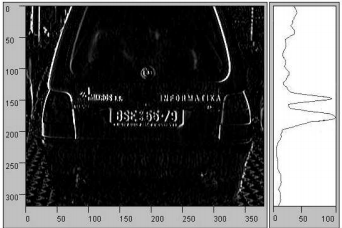
\includegraphics[scale=0.8]{histogram_after_edge_detection.png}  
    \caption{Вертикальная гистограмма после фильтра границ}
    \label{fig:domain:search:edges_analisys:vertical_histogram_after_edge_detection}
\end{figure}

Анализ гистограмм обрел большую популярность так как встречается сразу в нескольких работах ~\cite{recognition_using_histogram_1}~\cite{recognition_using_histogram_2}. 
Идея заключается в пред-обработке изображение фильтром границ с построением гистограммы в последующем. На рисунке \ref{fig:domain:search:edges_analisys:vertical_histogram_after_edge_detection} отчетливо виден всплеск на гистограмме в области автомобильного номера. Анализирую изменения на вертикальной и горизонтальной гистограмме можно вычислить положение автомобильного номера. 

Рассмотренный метод имеет достаточную производительность чтобы работать в режиме реального времени: при использовании компьютера с центральным процессором работающем на частоте 3.0 GHz и имеющем 512 MB оперативной памяти справлялся с обработкой изображения 320 на 240 пикселя в среднем 0.07 секунд.

Главным недостатком анализа гистограмм является существенное ограничение на входные данные: машина должны занимать значительную площадь на изображении и туда не должно попадать постороннего текста, который легко может стать причиной лишних всплесков на гистограмме.

\subsubsection{}
\label{sub:domain:search:violajones}
Метод Виолы - Джонса.

Метод Виолы - Джонса  это первый алгоритм обнаружения объектов работающий в режиме реального времени предложенный Paul Viola и Michael Jones в 2001 году~\cite{viola_jones_wiki}~\cite{viola_jones_habr}. Алгоритм использует компьютерное обучение с учителем и может быть обучен для распознавания различных объектов, во время разработки метода перед авторами стояла задача распознавание лица. 

Метод основан на следующих принципах:
\begin{itemize}
  \item Используются изображения в интегральном представлении, что позволяет вычислять быстро необходимые объекты;
  \item Используются признаки Хаара, с помощью которых происходит поиск нужного объекта;
  \item Используется бустинг для выбора наиболее подходящих признаков для искомого объекта на данной части изображения;
  \item Все признаки поступают на вход классификатора, который даёт результат «верно» либо «ложь»;
  \item Используются каскады признаков для быстрого отбрасывания окон, где не найдено лицо.
\end{itemize}

Для работы с изображением оно переводится в интегральное представление. Интегральное представление изображения это матрица, равная по размерам исходному изображению, в каждом элементе которой хранится сумма интенсивностей все пикселей находящихся левее выше данного элемента 
$$ L_{x,y} = \displaystyle\sum_{i=0}^{i<x} I_{i,j} $$.

\subsection{Распознавание символов}
\label{sub:domain:imagerecognition}
Для распознавания отдельного символа лучше всего использовать перцептрон.
Перцептрон — математическая или компьютерная модель восприятия информации мозгом (кибернетическая модель мозга)~\cite{perceptron}.
Перцептрон состоит из трёх типов элементов, а именно: поступающие от сенсоров сигналы передаются ассоциативным элементам, а затем реагирующим элементам. Таким образом, перцептроны позволяют создать набор ассоциаций между входными стимулами и необходимой реакцией на выходе.

Элементарный перцептрон состоит из элементов 3-х типов: S-элементов, A-элементов и одного R-элемента. S-элементы — это слой сенсоров, или рецепторов. В физическом воплощении они соответствуют, например, светочувствительным клеткам сетчатки глаза или фоторезисторам матрицы камеры. Каждый рецептор может находиться в одном из двух состояний — покоя или возбуждения, и только в последнем случае он передаёт единичный сигнал в следующий слой, ассоциативным элементам.

A-элементы называются ассоциативными, потому что каждому такому элементу, как правило, соответствует целый набор (ассоциация) S-элементов. A-элемент активизируется, как только количество сигналов от S-элементов на его входе превысило некоторую величину $\theta$. Таким образом, если набор соответствующих S-элементов располагается на сенсорном поле в форме буквы "Д", A-элемент активизируется, если достаточное количество рецепторов сообщило о появлении «белого пятна света» в их окрестности, то есть A-элемент будет как бы ассоциирован с наличием/отсутствием буквы "Д" в некоторой области.

Сигналы от возбудившихся A-элементов, в свою очередь, передаются в сумматор R, причём сигнал от i-го ассоциативного элемента передаётся с коэффициентом $w_i$. Этот коэффициент называется весом A—R связи.

Так же как и A-элементы, R-элемент подсчитывает сумму значений входных сигналов, помноженных на веса. R-элемент, а вместе с ним и элементарный перцептрон, выдаёт 1, если линейная форма превышает порог $\theta$ иначе на выходе будет -1. Математически, функцию, реализуемую R-элементом, можно записать так:
$f(x) = sign(\sum_{i=1}^{n} w_i x_i - \theta)$
Обучение элементарного перцептрона состоит в изменении весовых коэффициентов $W_i$ связей A—R. Веса связей S—A (которые могут принимать значения $\{ -1, 0, 1 \}$) и значения порогов A-элементов выбираются случайным образом в самом начале и затем не изменяются.

После обучения перцептрон готов работать в режиме распознавания или обобщения. В этом режиме перцептрону предъявляются ранее неизвестные ему объекты, и перцептрон должен установить, к какому классу они принадлежат. Работа перцептрон состоит в следующем: при предъявлении объекта, возбудившиеся A-элементы передают сигнал R-элементу, равный сумме соответствующих коэффициентов $w_i$. Если эта сумма положительна, то принимается решение, что данный объект принадлежит к первому классу, а если она отрицательна — то ко второму.

\subsection{Примеры реализации}
\label{sub:domain:realization}

\subsubsection{}
\label{sub:domain:realization:automarshal}
Автомаршал – программное обеспечение для распознавания номеров автомобилей. Применяется для автоматизации парковок, весовых, КПП, автомоек, ТСЖ и т.п.\cite{auto_marshal}
Достоинства:
\begin{itemize}
  \item Имеются версии распознающие номера на скорости до 150 км/ч
  \item Поддерживаются номерные знаки большого количества стран: Российская Федерация, Казахстан, Украина, Белоруссия, Киргизия, Узбекистан, Нидерланды, Польша, Бельгия, Германия
\end{itemize}
Недостатки:
\begin{itemize}
  \item Интегрируется только с *.xls, *.xlsx, *.csv базами данных, т.е не подходит для компаний с развитой IT инфраструктурой
  \item Высокая цена, которая зависи от количества камер и стран, чьи регистрационные знаки распознаются
  \item Работает только на \windows{} серверах.
  \item Нет возможности попробовать перед покупкой.
\end{itemize}

\subsubsection{}
\label{sub:domain:}
Модуль распознавания автомобильных номеров - Альфа системз~\cite{alpha_system}. Модуль распознавания автомобильных номеров автоматически определяет и распознает номера автомобилей в поле зрения камеры. Он позволяет фиксировать и сохранять в базе данных SQL распознанный номер, а также изображение транспортного средства, часть кадра с номерным знаком и время регистрации. Таким образом, формируется база всех транспортных средств, прошедших через зону контроля, с возможностью добавления текстового комментария к каждому распознанному номеру. В совокупности с модулем «Радар», предоставляющем информацию о скорости автомобилей, модуль распознавания автомобильных номеров может использоваться ГИБДД для регистрации нарушителей скоростного режима. Есть возможность сравнения распознаваемых номеров со сторонней базой номеров (например, автомобилей, числящихся в угоне), что позволяет применять модуль для целей розыска. Другим важным применением модуля является его использование в системах автоматического учета и контроля доступа автотранспорта на охраняемые объекты и платные автостоянки.
Достоинства:
\begin{itemize}
  \item Работает с SQL базами данных
  \item Поддерживаются номерные знаки большого количества стран: Российской Федерации, Беларуси, Украины, Молдавии, Казахстана, Узбекистана, Латвии, Эстонии, Польши, Германии, Испании, Бразилии, Кубы.
\end{itemize}
Недостатки:
\begin{itemize}
  \item Возможность интеграции лучше чем у Автомаршала(\ref{sub:domain:realization:automarshal}) но все ещё не достаточно хороша: нет точки расширения для интегрирования с имеющимися rest сервисами компании.
  \item Высокая и непрозрачная цена.
  \item Работает только на \windows{} серверах.
  \item Нет возможности попробовать перед покупкой.
\end{itemize}

\subsubsection{}
Распознаватель авто номеров - autonomerok. Autonomerok - производит распознавание номера машины в потоке, сохранение события с записью номера, времени и кадра с номером, а также может управлять исполнительными устройствами. Программа будет отлично работать c аналоговыми IP видеокамерами разных производителей.
\begin{itemize}
  \item Работает с SQL light базой данных.
  \item Есть возможность проверить перед покупкой.
\end{itemize}
Недостатки:
\begin{itemize}
  \item Возможность интеграции лучше чем у Автомаршала(\ref{sub:domain:realization:automarshal}) но все ещё не достаточно хороша: нет точки расширения для интегрирования с имеющимися rest сервисами компании.
  \item Высокая цена.
  \item Работает только на \windows{} серверах.
  \item Небольшая количество по сравнению с Автомаршалом и Альфи системз, количество поддерживаемых типов номерных знаков.
\end{itemize}

\subsubsection{} Все имеющиеся приложения имеют высокую цену и лишний для нашей задачи функционал. Они позиционирую себя как готовые решения для платных парковок, авто моек и т.п. и расчитаны больше на малые компании и частных предпринимателей, у которых нет развитой IT инфраструктуры. 

\subsection{Постановка целей и задач дипломного проекта}
Цель - разработка программного средства для автоматизации автомобильной стоянки компании \company{}.


Задачи:
\begin{itemize}
  \item Разработка архитектуры ПС;
  \item Разработка алгоритмов;
  \item Выбор платформы для разработки программного средства;
  \item Разработка пользовательского интерфейса;
  \item Создание базового проекта в среде программирования;
  \item Создание пользовательского интерфейса;
  \item Программирование и тестирование модулей;
  \item Сборка и тестирование ПС;
\end{itemize}
